\documentclass{article}
\usepackage[margin=1in]{geometry}
\usepackage{braket}
\usepackage{amsmath}
\usepackage{graphicx}
\graphicspath{ {./figures} }

\begin{document}

\title{Revised algorithm description section}
\maketitle

\section{ISA framework, formal description and implementation}
In this work, we propose an approximate quantum state preparation framework,
which we call ``Iterative Sparse Approximation" (ISA). Let the target state be
$\ket{x_0}$. Then the ISA framework transforms $\ket{x_0}$ to 
$\ket{x_1}$, then $\ket{x_1}$ to $\ket{x_2}$, and so on, until it reaches some
state $\ket{x_m}$, such that
$$|\braket{0|x_0}|^2 < |\braket{0|x_1}|^2 < ... < |\braket{0|x_m}|^2$$
And
$$|\braket{0|x_m}|^2 \geq 1 - \epsilon$$
Each transformation from $\ket{x_i}$ to $\ket{x_{i + 1}}$ generates a state
closer to $\ket{0}$; these steps are called ``refinements." The sequence 
of gates used in each refinement step are combined to create the 
state preparation sequence for $\ket{x_0}$.

To refine $\ket{x}$, the
ISA framework selects an index subset $K \subset \{0,,,2^n - 1\}$ 
and constructs the sparse, usually non-normalized approximation
$$\ket{x} \approx \ket{x'} = \sum_{k \in K}{\braket{k | x}}$$
If $\ket{x} = \sum_{i=0}^{2^n - 1}{c_i \ket{i}}$, then 
$\ket{x'} = \sum_{k \in K}{c_k\ket{k}}$, showing that $\ket{x'}$ has at
most $|K|$ non-zero elements and is therefore sparse.

Next, the sparse state preparation method for $\ket{x'}$
is adapted towards the refinement of $\ket{x}$. Because $\ket{x'}$
approximates $\ket{x}$, the state preparation sequence for 
$\ket{x'}$ approximately prepares $\ket{x}$. However, $\ket{x'}$ and 
$\ket{x}$ are not the same state, motivating the need for an adaptation step.
Index subset selection $K$ (``Select"), constructing and preparing $\ket{x'}$ 
(``Prepare"), and adapting the state preparation sequence for $\ket{x'}$ to 
refine $\ket{x}$ (``Adapt") constitute the central steps in the ISA framework,
as shown in Algorithm 1.

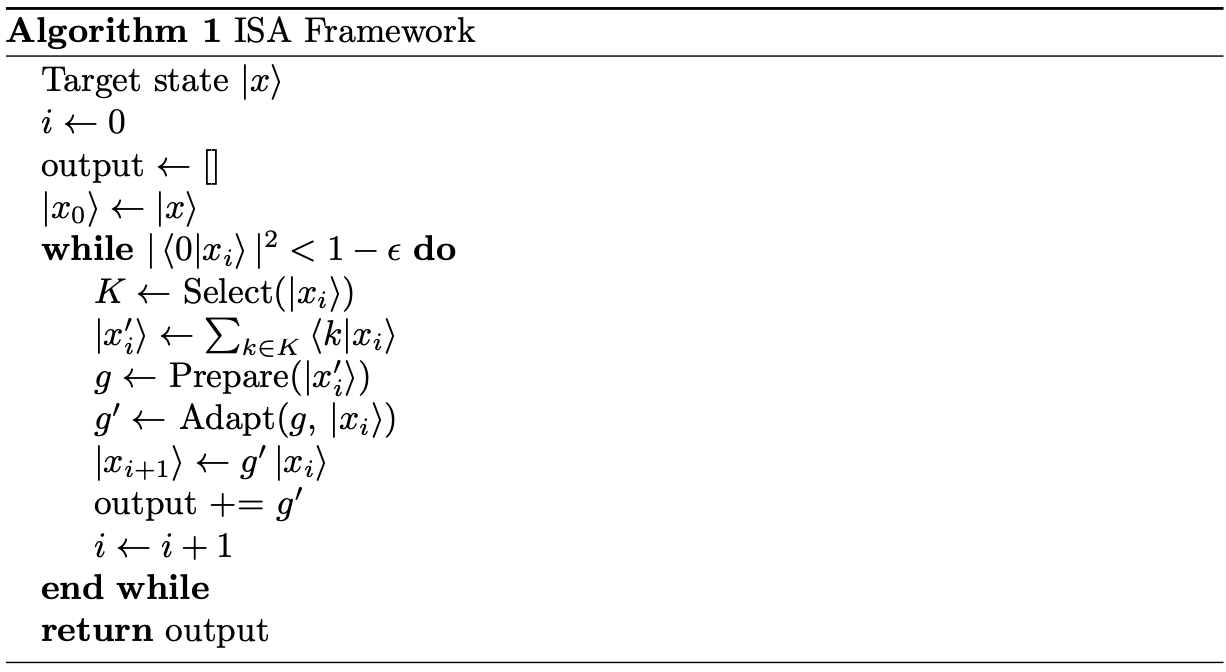
\includegraphics[width=0.8\textwidth]{isa_algo}

In the remainder of this
section, we describe our specific implementation of the ISA framework for linear
nearest neighbor architectures. In section x.1, we describe the two types of
index subsets $K$ considered for the Select step, as well as the procedure for
choosing one. In section x.2, we describe our implementation of the Prepare step
for each index subset type. In section x.3, describe our implementation of the
Adapt step. Finally, in section x.4, we describe an additional step in our 
implementation, 
called ``Refinement by RZ-RY," in which the starting state $\ket{x_0}$ is first
refined to $\ket{x_1}$ using RZ and RY gates before applying the ISA framework.

\subsection{Index subsets and implementing Select}
Type 1 index subsets are those of the form:
$$K(b) = \{0, b\}$$
For some $b$ between 1 and $2^n - 1$ inclusive.

Type 2 index subsets take one of two different forms:
$$K^{(+)}(a, p) = \{a * 2^{p + 2} + i * 2^p | 0 \leq i \leq 3\} \cup \{i * 2^p | 0 \leq i \leq 3\}$$
$$K^{(-)}(a, p) = \{a + i * 2^p | 0 \leq i \leq 3\} \cup \{i * 2^p | 0 \leq i \leq 3\}$$
For some $a$ and $p$. For the $K^{(+)}$ case, $0 \leq a \leq 2^{n - p - 2} - 1$;
in the $K^{(-)}$ case, $0 \leq a \leq 2^p - 1$. In both cases, $0 \leq p \leq n - 2$.
When written in binary, the indices in $K^{(+)}$ subsets are those where the
left-most $n - p - 2$ bits are either $a$ or zeroes, the right-most $p$ bits are
zeroes, and the middle two bits can be any length-2 bitstring, and the indices 
in $K^{(-)}$ subsets are those where the left-most $n - p - 2$ bits are zeroes,
the right-most $p$ bits are either $a$ or zeroes, and the middle two bits can be
any length-2 bitstring. 

When refining a state $\ket{x}$, each subset $K$ corresponds to a non-normalized
sparse approximation $\ket{x'(K)}$. Let CX\_count($K$) be the number of CX gates
required to prepare $\ket{x'(K)}$. Then, at the Select step, we choose the index
subset $K$ that maximizes the fidelity increase ratio:
$$\text{fidelity increase ratio}(K) = \frac{\braket{x'(K)|x'(K)} 
- |\braket{0|x}|^2}{\text{CX\_count}(K) + 1}$$
This quantity is named ``fidelity increase ratio" because if $\ket{y(K)}$ is the
state after applying the state preparation sequence of $\ket{x'(K)}$ to 
$\ket{x}$, then $|\braket{0|y(K)}|^2 = \braket{x'(K)|x'(K)}$, corresponding to a
fidelity increase of $|\braket{0|y(K)}|^2 - |\braket{0|x}|^2 
= \braket{x'(K)|x'(K)} - |\braket{0|x}|^2$. This improvement is divided by the 
number of CX gates required to achieve it to compute the fidelity increase per
CX gate; +1 is added to the denominator to prevent division by zero. Thus, at
each step, $K$ is chosen to maximize the projected fidelity increase per CX
gate applied.

\subsection{Implementing Prepare}
Type 1 and Type 2 index subsets give rise to Type 1 and Type 2 sparse quantum
states. Our preparation method for these states is an extension of 
[Gleinig and Hoefler] for limited connectivity architectures.

Type 1 index subsets give rise to quantum states of the form
$$\ket{x'(b)} = c_0\ket{0} + c_b\ket{b}$$
For some $b > 0$ and complex amplitudes $c_0$ and $c_b$. 
To prepare such states, a sequence
of CX gates, $g_1g_2...g_l$ is used to move $\ket{b}$ to a sequence of other
basis states, $\ket{b_1}$, $\ket{b_2}$, ..., $\ket{b_l}$ such that
$$g_i\ket{b_{i - 1}} = \ket{b_i} \quad \text{for all} \quad 1 \leq i \leq l, b_0 = b$$
$$b_l = 2^j \quad \text{for some } j$$
CX gates leave $\ket{0}$ unchanged, therefore, this sequence of CX gates
transforms $\ket{x'(b)}$ to a new state:
$$\ket{x''} = c_0\ket{0} + c_b\ket{2^j}$$
Which is a one-qubit state, and can be prepared using an RZ and RY gate [ref].
Let $CXD(b) = l$ be the minimum number of CX gates required to prepare 
$\ket{x'}$;
the formula for $CXD(b)$ is presented in the Appendix. Then, each CX gate $g_i$
can be computed by selecting a CX gate such that $CXD(b_i) = CXD(b_{i-1}) - 1$.

The Type 2 index subsets $K^{(+)}(a, p)$ give rise to Type 2 quantum states of
the form:
$$\ket{x'^{(+)}(a, p)} = (\ket{a} \otimes \ket{\psi_1} + \ket{0} \otimes \ket{\psi_2}) \otimes \ket{0_p}$$.
Where $\ket{\psi_1}$ and $\ket{\psi_2}$ are non-normalized, two-qubit states and
$\ket{0_p}$ represents all zeroes in the lowest $p$ qubits. To prepare such
states, a sequence of CX gates, $g_1g_2...g_m$ are applied to the upper 
$n - p - 2$ qubits to transform 
$\ket{a}$ to a sequence of other basis states, 
$\ket{a_1}$, $\ket{a_2}$, ..., $\ket{a_m}$ such that
$$g_i\ket{a_{i - 1}} = \ket{a_i} \quad \text{for all} \quad 1 \leq i \leq m, \ket{a_0} = \ket{a}$$
$$\ket{a_m} = \ket{1}$$
Again, CX gates leave $\ket{0}$ unchanged, so this sequence transforms $\ket{x'^{(+)}(a, p)}$ to
$$\ket{x''^{(+)}} = (\ket{1} \otimes \ket{\psi_1} + \ket{0} \otimes \ket{\psi_2}) \otimes \ket{0_p}$$
The result is a three-qubit state, which can be prepared exactly using three CX
gates [ref]. We give our construction for linear nearest neighbor architectures
in the Appendix. In addition, let $CXD^{(+)}(p) = m$ be the minimum number of
CX gates required to transform $\ket{a}$ to $\ket{1}$; the formula for 
$CXD^{(+)}$ is given in the Appendix.

In the special case where $a = 0$, the index subset $K^{(+)}(a, p)$ gives rise
to a two qubit state:
$$\ket{x'} = \ket{0_{n - p - 2}} \otimes \ket{\psi_0} \otimes \ket{0_p}$$
Which can be prepared using one CX gate [ref].

The Type 2 index subsets $K^{(-)}(a, p)$ give rise to quantum states of the form
$$\ket{x'^{(-)}(a, p)} = \ket{0_{n-p-2}} \otimes (\ket{\psi_1} \otimes \ket{a} + \otimes \ket{\psi_2} \otimes \ket{0})$$
Where $\ket{\psi_1}$, $\ket{\psi_2}$, and $\ket{0_{n-p-2}}$ are defined as in
the $K^{(+)}(a, p)$ case. Note that these states are the same as those in 
[ref equation], but with the qubits in reverse order. Thus, the same state
preparation method applies to this case.
\subsection{Implementing Adapt}
If $K$ is a Type 1 index subset, then the corresponding sparse approximation
takes the form
$$\ket{x'} = c_0\ket{0} + c_b\ket{b}$$.
And the state preparation method involves applying CX gates to move $\ket{b}$ to
$\ket{2^i}$, before applying a one-qubit state preparation procedure. To adapt
this to refining $\ket{x}$, we re-imagine the process of moving $\ket{b}$ using
CX gates as an iterative merging procedure using CX, RZ, and RY gates. If $b$
and $b'$ are two length-$n$ bitstrings that differ in only the $i$th bit and
both $b$ and $b'$ have a 1 at position $j$ for $|i - j| = 1$, then
the amplitude at $\ket{b}$ can be merged into the amplitude at $\ket{b'}$ using
the following procedure:

[subroutine description]

Granted, this procedure will generally shuffle the amplitudes of many other
bases, but it leaves the amplitude at $\ket{0}$ unchanged (up to a phase). Then,
the procedure for adapting $\ket{x'}$ for refining $\ket{x}$ is:

[Refinement by ISA, Type 1]

At each iteration, the algorithm constructs a list of all possible CX gates that
modify $\ket{b}$. For each propective CX gate, the projected fidelity increase
ratio is updated, and the maximal fidelity increase ratio is selected.

\subsection{Refinement by RZ-RY}
Copy and paste from original text?
then

Our specific implementation of the ISA framework is summarized in Algorithm 2.
[pseudo-code for specific ISA implementation].
\end{document}


